\subsection{Barrel Micromegas Tracker (BMT)}

\subsubsection{Geometry}

The Micromegas geometry is implemented through the native GEMC geometry API.
There are three micromegas regions, divided azimuthally in three identical sectors. Each sector contain a cover layer with copper ground,
the PCB with the readout strips, the kapton support, the mesh layer and the ionizing gas:

\begin{itemize}
	\item -- overlay
	\item ---- copper ground
	\item ------ pcb
	\item -------- strips
	\item ---------- kapton
	\item ------------ gas (amplification gap)
	\item -------------- mesh
	\item ---------------- gas (drift detection gap)
	\item ------------------ drift potential electrode
	\item -------------------- foil
	\item ---------------------- ground
\end{itemize}

The sensitive volume containing the gas is assigned the argon isobutan gas and associated with the BMT hit process routine.
The geometry is summarized in \F{bmtGeometry}

The strip identification is performed in the Process ID routine.

\begin{figure}
	\centering
	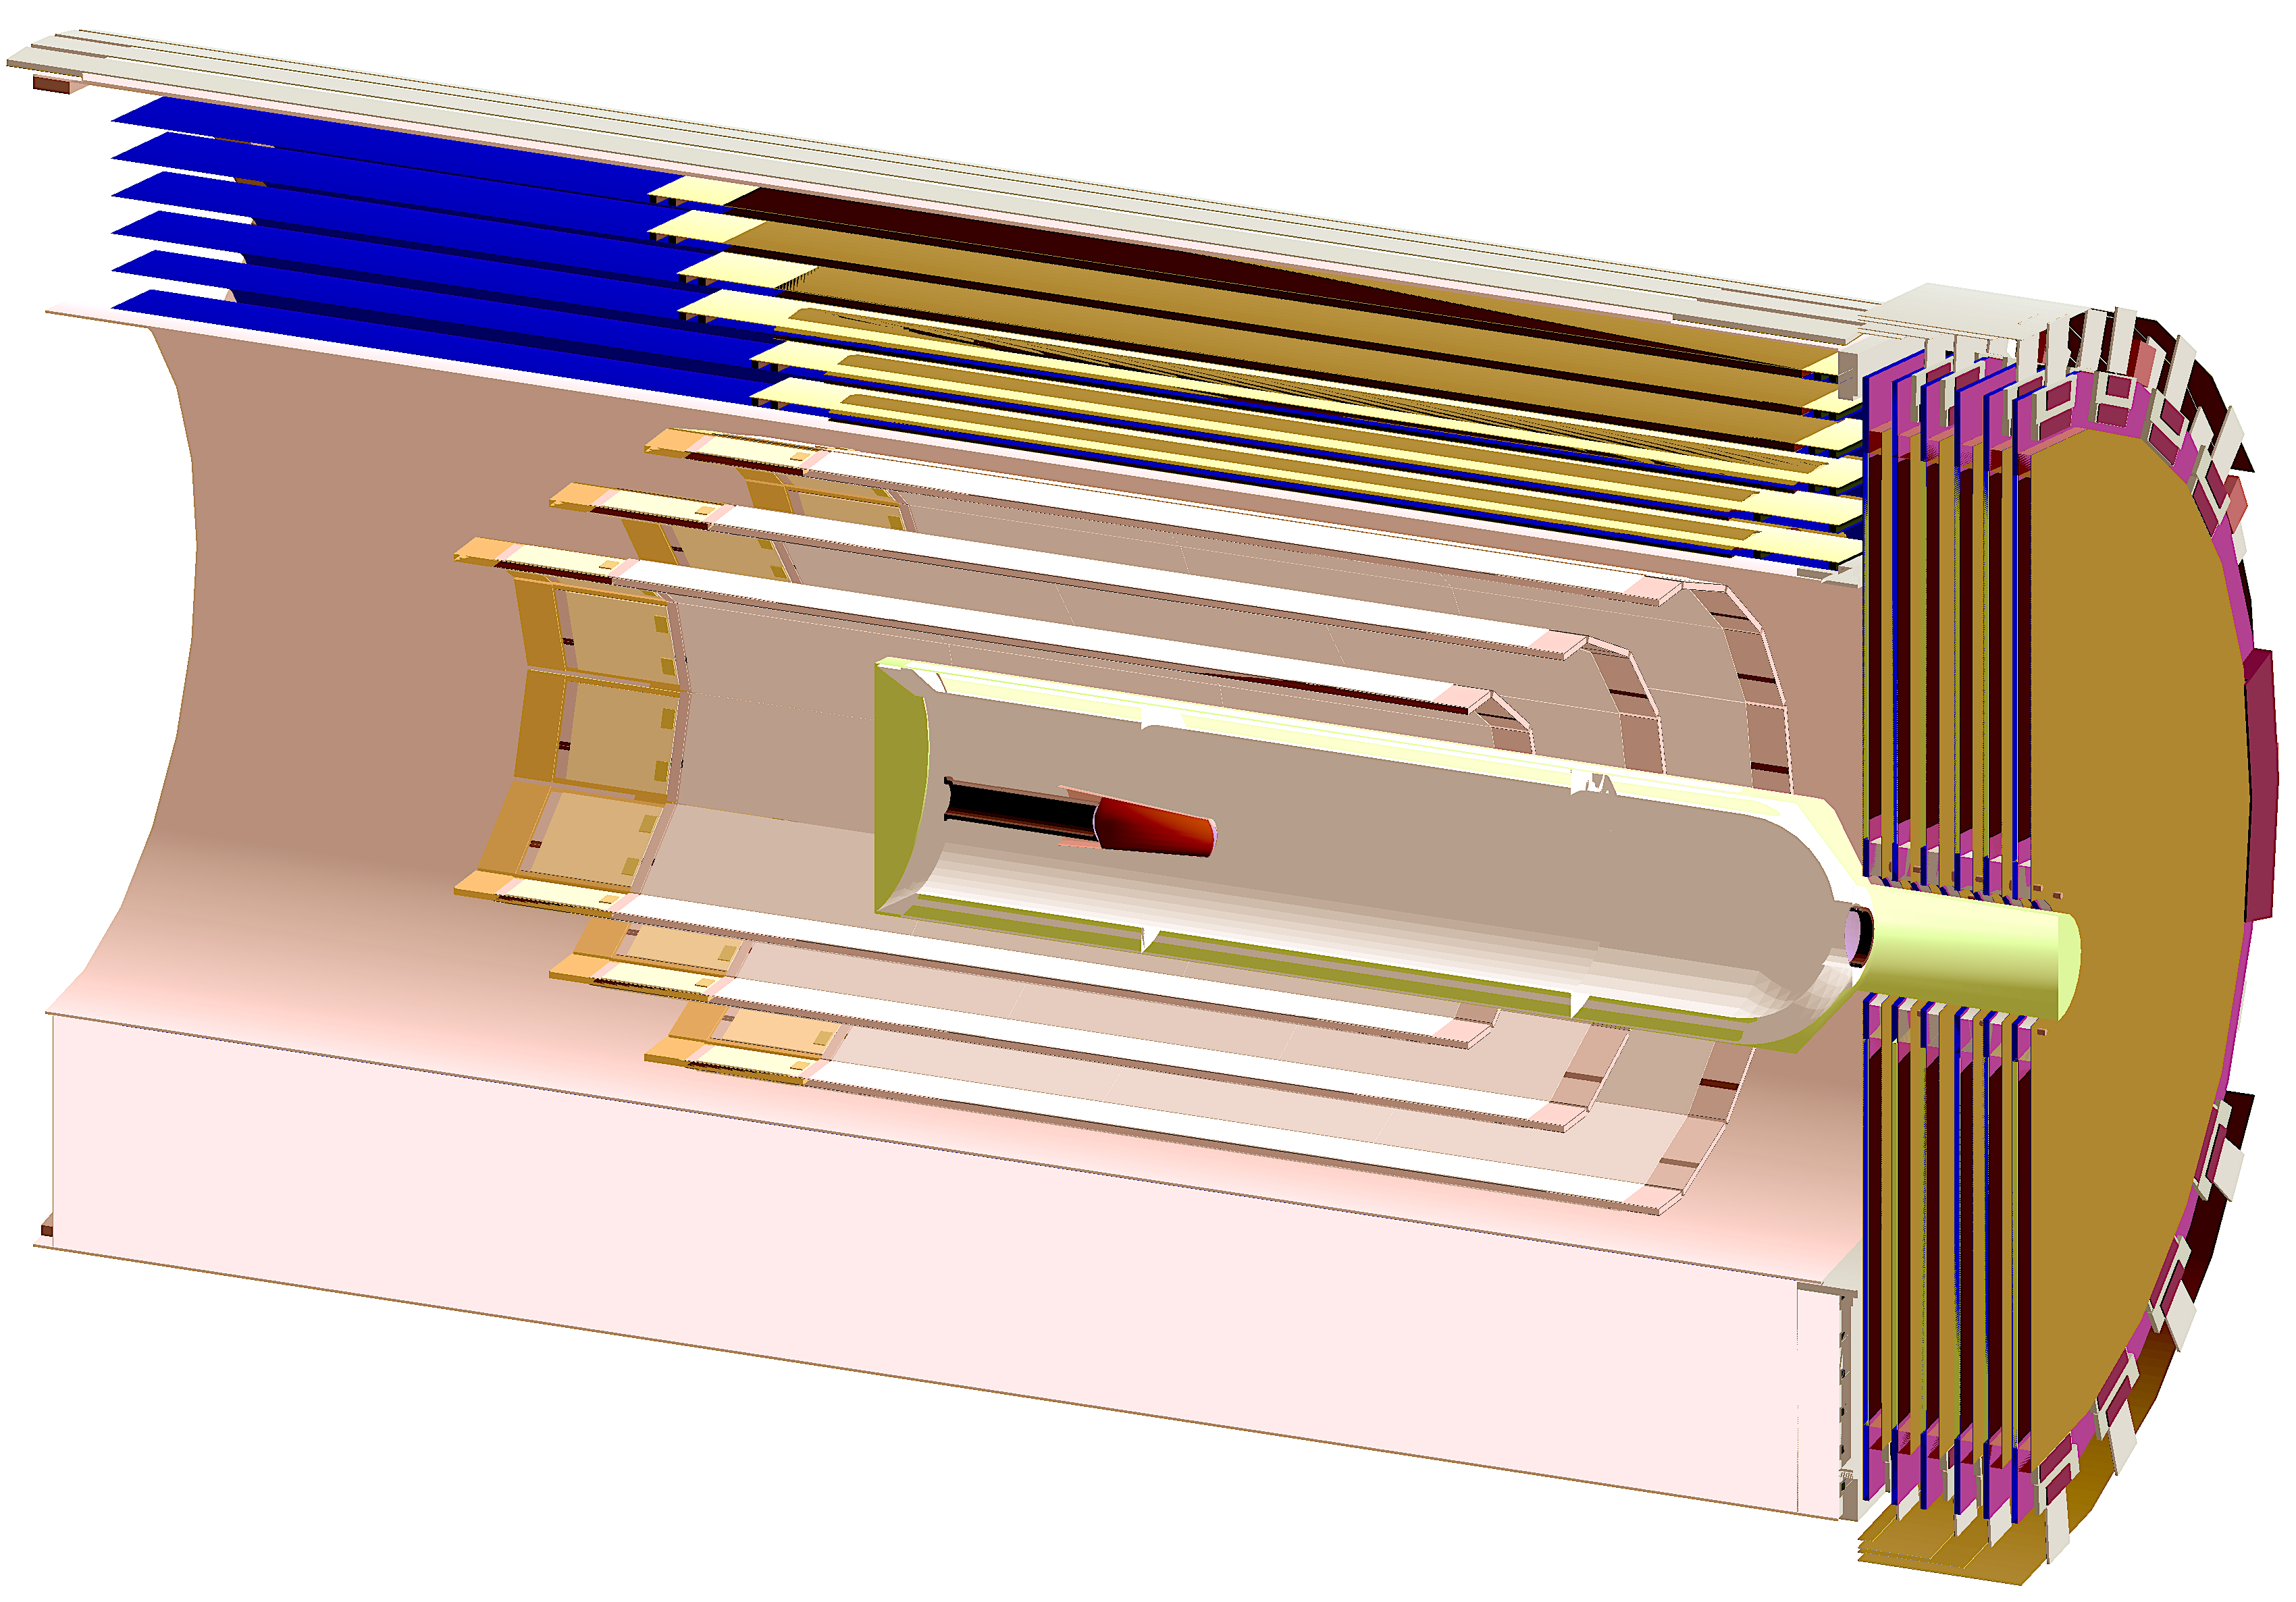
\includegraphics[width=0.95\columnwidth,keepaspectratio]{img/bmtGeometry.png}
	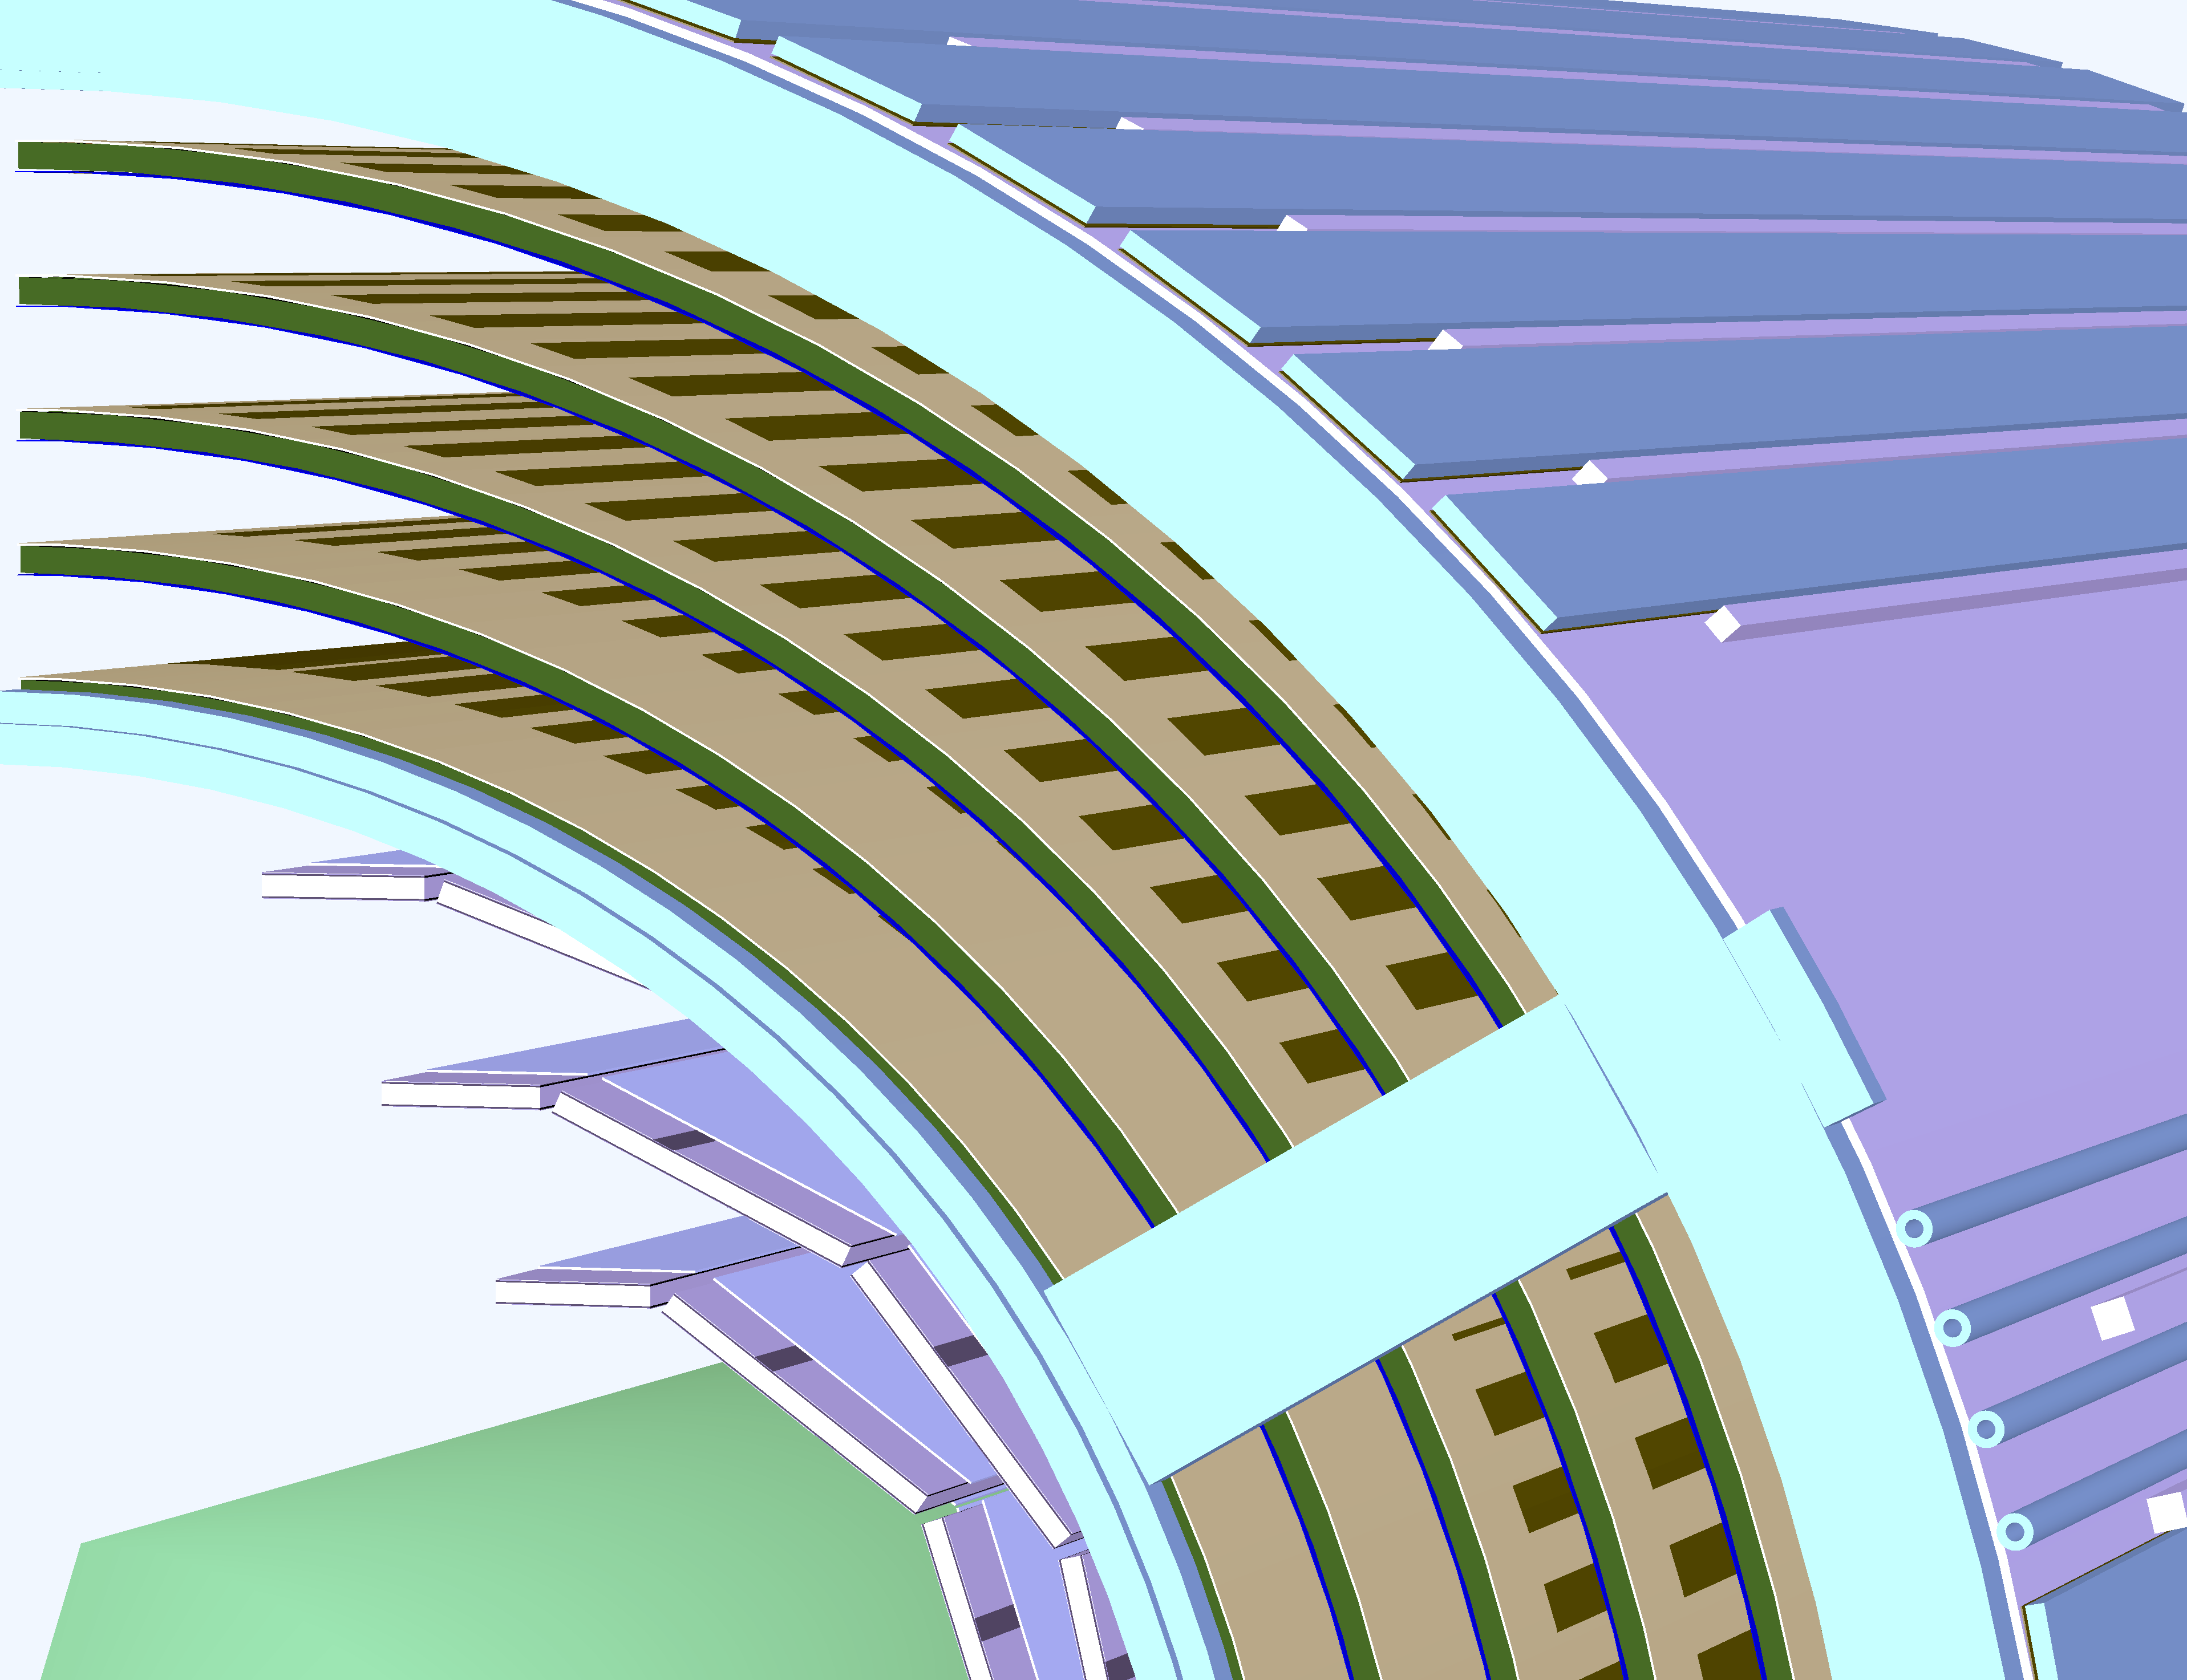
\includegraphics[width=0.95\columnwidth,keepaspectratio]{img/bmtDetail.png}
	\caption{Top: an overall view of the central detector trackers. The target is surrounded by 3 layers of silicon vertex trackers and
            6 layers of micromegas, 3 with Z-trips, 3 with C-strips. On the front the Forward Micromega Tracker disks are visible.
            Bottom: detail of the micromegas GEMC geometry, showing the overlay cover, the copper ground and pcb strips}
	\label{fig:bmtGeometry}
\end{figure}



\subsubsection{Geometry Location on GitHub}
The Github location of the GEMC perl API script is \url{https://github.com/gemc/detectors/tree/master/clas12/micromegas}.


\subsection{Process ID}
At each Geant4 step, the local coordinate in the sensor volume are used to calculate the strip id.
The algorithm includes the Lorentz angle based on the magnetic field strength, the particle direction, pitch between the strips,
the dead zones of the sensitive parts. A virtual electron avalanche is simulated based the energy deposited. The avalanche
is deposited onto one strip or distributed among several to account for the energy sharing.



\subsection{Digitization}

\subsubsection{ADC}
The Micromegas digitization provides the ADC value calculated using the total energy deposited (after hit sharing).


\subsubsection{TDC}
There is no timing information in the output.

\subsubsection{Summary of CCDB Table Used}

\begin{itemize}
	\item /geometry/cvt/mvt/bmt\_layer\_noshim
	\item /geometry/cvt/mvt/bmt\_strip\_L1
	\item /geometry/cvt/mvt/bmt\_strip\_L2
	\item /geometry/cvt/mvt/bmt\_strip\_L3
	\item /geometry/cvt/mvt/bmt\_strip\_L4
	\item /geometry/cvt/mvt/bmt\_strip\_L5
	\item /geometry/cvt/mvt/bmt\_strip\_L6
\end{itemize}


\subsection{Digitized Bank}
The digitized output bank has $ID=500$, and the variables are summarized in Table \ref{tab:mmBank}.

\begin{table}[h]
	\begin{center}
		\begin{tabular}{| c | c | c |}
			\hline \hline
			Variable         & Description  & Tag  \\
			\hline
              layer  &                                      layer number  &    1   \\
             sector  &                                     sector number  &    2   \\
              strip  &                                      strip number  &    3   \\
               Edep  &                                  energy deposited  &    4   \\
                ADC  &                                               ADC  &    5   \\
			\hline \hline
		\end{tabular}
	\end{center}
	\caption{The digitized micromegas bank.}\label{tab:mmBank}
\end{table}

\subsubsection{Time Window}
The time window  of the Micromegas is set to to 132 ns.

\subsubsection{Process Routine Git Repository Location}
The BST hit process routines are located in the repository: \url{https://github.com/gemc/source/tree/master/hitprocess/clas12/micromegas}

